\documentclass[11pt]{report}

\usepackage{graphicx}

\newcommand{\define}[2] {
  \textbf{Definition: #1}
  \begin{center} #2
\end{center}
}

\begin{document}

\title{PMR lecture notes}
\maketitle
\tableofcontents

\chapter{Belief networks}
\begin{figure}[H]
\centering
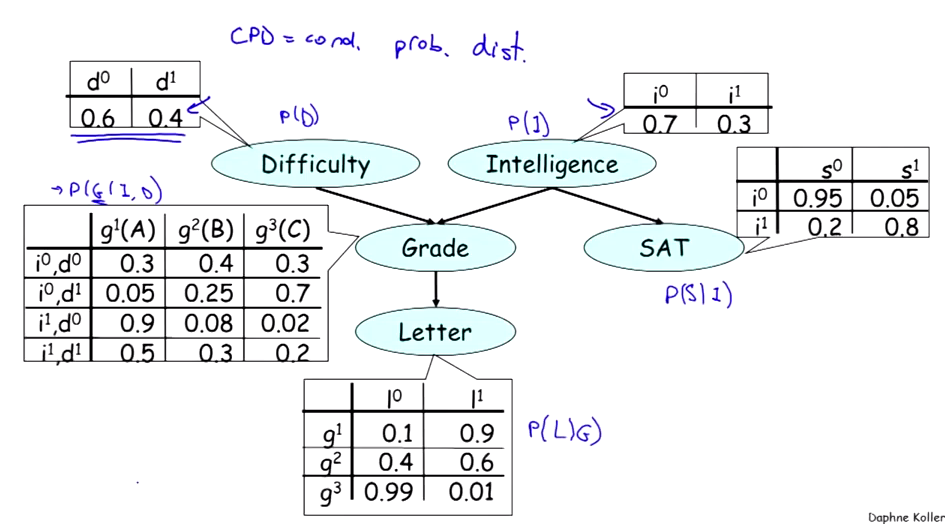
\includegraphics[width=90mm]{images/cpd_bayesnetwork.png}
\caption{Effects of multiple objects creating sound}
\label{sensorymockup2}
\end{figure}


\section{Questions}

\end{document}